\documentclass{beamer}

\usepackage{mytheme}

% For Title Page
% ---------------------------------------------------------------------------------------

\title{Applications of Galois Theory}

\author[Sandesh Thakuri]{Mr. Sandesh Thakuri}

\institute[CDM, TU]
{Central Department of Mathematics, TU}

\date{2081-1-9}


% Begin Document
% ---------------------------------------------------------------------------------------------------------------------

\begin{document}
\myfootline

\begin{frame}[plain]
  \tikzonlytitlepage
  \titlepage
\end{frame}

\begin{frame}[plain]
\begin{figure}[h!]
  \centering
  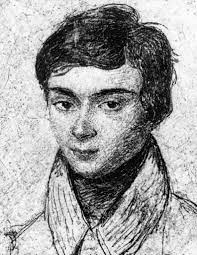
\includegraphics[width=4cm, height=3.5cm]{galois.jpg}
  \caption{\footnotesize Portrait of Galois}
\end{figure}

In my thesis, I have \textcolor{violet}{explored the applications} of Galois Theory in both pure and applied mathematics. Modern Galois Theory is the theory of field extension. \\
\textcolor{green!50!black}{The foundation of this theory was laid by the French Mathematician \textit{Évariste Galois} in the 1800s who had died at the early age of 20.}
\end{frame}

\begin{frame}[plain]
  \begin{tcolorbox}[colframe=blue!80!violet, colback=white, boxsep=3mm,  title={ \large \bfseries Outlines}]
    \vspace{3mm}
    \tableofcontents
  \end{tcolorbox}
\end{frame}

% -----------------------------------------------------------------------------------------------------------------------
\small
\section{Galois Theory}

\subsection{Galois Correspondence}
\begin{frame}{Background}

 Let \(F\) be an extension field of a field \(K\).
  \vspace{5mm}

  \begin{tcolorbox}[colframe=blue!40, colback=white, boxsep=1mm]
    \begin{definition} [Galois Group]
      The set of all \textcolor{magenta}{automorphisms} of \(F\) that fixes \(K\) element-wise forms a permutation group.\\[2mm]
      This group is called the Galois group of \(F\) over \(K\) and it is denoted by \(Aut_K^F\) \cite{hunger}.
    \end{definition}
    \vspace{4mm}
    \begin{definition}[Galois Extension]
      The extension field \(F\) of \(K\) is said to be Galois extension if the fixed field of the Galois group \(Aut_K^F\) is \(K\) itself.
    \end{definition}
  \end{tcolorbox}
\end{frame}

\begin{frame}{Galois Correspondence}
    \begin{tcolorbox}[colback=white, colframe=blue!40, boxsep=1mm]
  \begin{theorem}[Fundamental Theorem of Galois Theory]
  If \(F\) is a finite dimensional Galois extension of \(K\), then there is a \textcolor{magenta}{one-to-one correspondence between the set of all intermediate fields of \(F\) over \(K\) and the set of subgroups of the Galois group \(Aut_K^F\)} such that:
  \begin{enumerate}
  \item[i)] the relative dimension of two intermediate fields is equal to the relative index of the corresponding subgroups. In particular \(Aut_K^F\) has order \([F:K]\);
  \item[ii)] \(F\) is Galois over every intermediate field \(E\), but \(E\) is Galois over \(K\) if and only if the corresponding subgroup \(E'= Aut_E^F\) is normal in \(G=Aut_K^F\). In this case \(G/E'\) is isomorphic to the Galois group \(Aut_K^E\) of \(E\) over \(K\) \cite{hunger}.
  \end{enumerate}
\end{theorem}
\end{tcolorbox}
\vspace{2mm}
\textcolor{green!40!black}{This theorem connects Field Theory to Group Theory.}
\end{frame}

\begin{frame}{Illustration of The Fundamental Theorem}
  \begin{minipage}{0.65\textwidth}
  Let \(F\) be an Galois extension of a field \(K\) and \(E\) be the intermediate field of \(F\) over \(K\):
  \[
    K \subset E \subset F
  \]
\noindent
  Let \(G\) be the Galois group of \(F\) over \(K\). Then \(H\) and \({e}\) are its subgroups:
  \[
    \{e\} \subset H \subset G
  \]
  Then the \textcolor{violet}{one-to-one correspondence} is as shown:
\end{minipage}
\begin{minipage}{0.3\textwidth}

  \begin{tcolorbox}[colback=white, colback=orange!20, colframe=orange!80!black, title={\footnotesize \textcolor{white}{Galois-correspondence}}, width=4cm]
    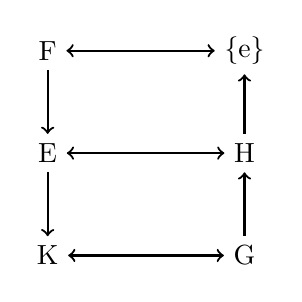
\begin{tikzpicture}
      \node (f) {F};
      \node[below of=f, yshift=-3mm] (e) {E};
      \node[below of=e, yshift=-3mm] (k) {K};

      \draw[->,thick] (f)--(e);
      \draw[->,thick] (e)--(k);

      \node[right of=f, xshift=15mm] (i) {\{e\}};
      \node[below of=i, yshift=-3mm] (h) {H};
      \node[below of=h, yshift=-3mm] (g) {G};

      \draw[<-, thick] (i)--(h);
      \draw[<-, thick] (h)--(g);

      \draw[<->, thick] (f)--(i);
      \draw[<->, thick] (e)--(h);
      \draw[<->, thick] (k)--(g);
    \end{tikzpicture}
  \end{tcolorbox}
\end{minipage}

\vspace{5mm}

 \begin{tcolorbox}[colback=white, colframe=blue!40, boxsep=0mm]
\begin{definition}[Remark]
  The intermediate fields are getting larger as we go from bottom to top  as the fields are getting extended. But the subgroups are getting smaller.
\end{definition}
\end{tcolorbox}
\end{frame}

\begin{frame}{Nature of Number}
  \textcolor{magenta}{The nature of a number depends upon the underlying field.}\\
  \(\sigma: \{a + b\sqrt{2}\} \mapsto \{a - b\sqrt{2}\} \) denoted by \(\sqrt{2} \longmapsto -\sqrt{2}\) is an automorphism of the field \(\mathbb{Q}(\sqrt{2})\) that fixes \(\mathbb{Q}\). So,  any polynomial equation over \(\mathbb{Q}\) satisfied by the number \(\sqrt{2}\) is also satisfied by the number \(-\sqrt{2}\). You can fluidly pass between these two numbers and the equation with a rational coefficient will not know. \textcolor{green!50!black}{Hence the two numbers \(\sqrt{2}\) and \(-\sqrt{2}\) are algebraically same over \(\mathbb{Q}\).}\\[4mm]

But the map \(\sqrt{2} \longmapsto -\sqrt{2}\) does not fix  \(\mathbb{Q}(\sqrt{2})\) i.e doesn't fix itself. So, you cannot pass \(\sqrt{2}\) for \(-\sqrt{2}\) for every equation with coefficients in \(\mathbb{Q}(\sqrt{2})\). \textcolor{green!50!black}{Hence the two numbers \(\sqrt{2}\) and \(-\sqrt{2}\) are not algebraically same over \(\mathbb{Q}(\sqrt{2})\).}
\vspace{2mm}

\begin{figure}[h]
  \centering
 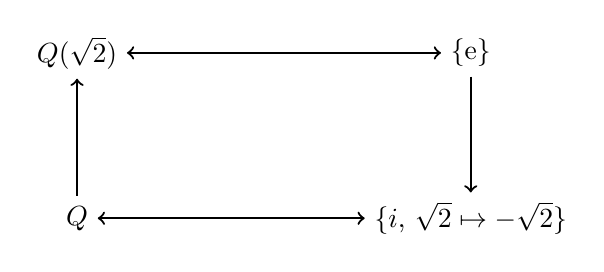
\begin{tikzpicture}
      \node (f) {\(\mathbb{Q}(\sqrt{2})\)};
      \node[below of=f, yshift=-11mm] (e) {\(\mathbb{Q}\)};


      \draw[<-,thick] (f)--(e);

      \node[right of=f, xshift=40mm] (i) {\{e\}};
      \node[below of=i, yshift=-11mm] (h) {\{\(i\), \(\sqrt{2} \mapsto -\sqrt{2}\)\}};


      \draw[->, thick] (i)--(h);


      \draw[<->, thick] (f)--(i);
      \draw[<->, thick] (e)--(h);
    \end{tikzpicture}
  \end{figure}
\end{frame}

\begin{frame}{Structure of a Field}
  The structure of a field as an extension field over some field is mirrored in the structure of the ``group'' of  permutations of its elements that keeps the base field fixed. But these permutations are the symmetries of the field. \textcolor{magenta}{So, the structure of field extension is equals to its own symmetry.}\\[2mm]

The structure of a field is a \textcolor{green!50!black}{complicated} thing; specially if it is infinite. But the structure of a group is rather \textcolor{green!50!black}{simple}; especially if it is finite. So the Galois theory has fairly simplified the complicated thing in a very insightful and beautiful way.

\vspace{3mm}
\begin{figure}[h]
  \centering
  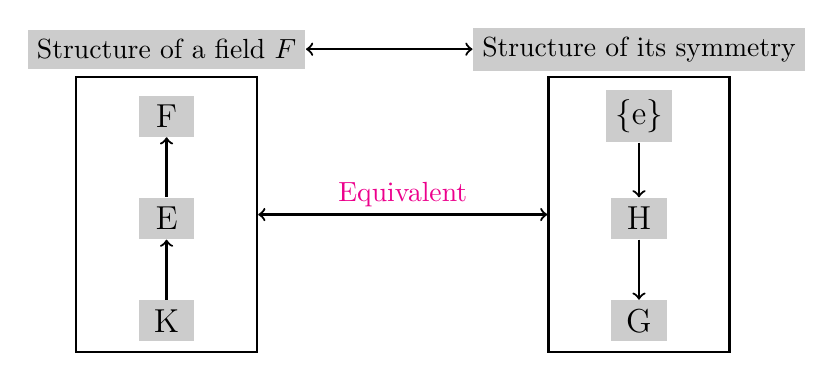
\begin{tikzpicture}

    \node[rectangle, thick, draw,
    minimum height=3.5cm,
    minimum width=2.3cm] (rec) at (0,0) {};

    \node[rectangle, thick, draw,
    minimum height=3.5cm,
    minimum width=2.3cm] (rec2) at (6,0) {};


    \node[minimum width=7mm,
      minimum height=5mm,
      fill=gray!40,
      ] (ss) at (0,2.1) {Structure of a field \(F\)};

      \node[minimum width=7mm,
      minimum height=5mm,
      fill=gray!40,
      ] (ss2) at (6,2.1) {Structure of its symmetry};

      \draw[<->, thick] (ss)--(ss2);
       \draw[<->, thick] (rec)--(rec2);

      \node[minimum width=7mm,
      minimum height=5mm,
      fill=gray!40] (f) at (0,1.25) {\large F};

      \node[minimum width=7mm,
      minimum height=5mm,
      fill=gray!40,
      below of=f, yshift=-3mm] (e) {\large E};

      \node[right of=e,
      xshift=20mm, yshift=3mm] (txt) {\textcolor{magenta}{Equivalent}};

      \node[minimum width=7mm,
      minimum height=5mm,
      fill=gray!40,
      below of=e, yshift=-3mm] (k) {\large K};

      \draw[<-,thick] (f)--(e);
      \draw[<-,thick] (e)--(k);

      \node[right of=f,
      xshift=5cm,
      minimum width=7mm,
      minimum height=5mm,
      fill=gray!40,
      ] (i) {\large \{e\}};

      \node[minimum width=7mm,
      minimum height=5mm,
      fill=gray!40,
      below of=i, yshift=-3mm] (h) {\large H};

      \node[
      minimum width=7mm,
      minimum height=5mm,
      fill=gray!40,
      below of=h, yshift=-3mm] (g) {\large G};

      \draw[->, thick] (i)--(h);
      \draw[->, thick] (h)--(g);
    \end{tikzpicture}
\end{figure}

  \end{frame}

\subsection{Structure of Galois Extension}
\begin{frame}{Question}
  Galois extension \(F\) of  \(K\) is a field for which the fixed field of the Galois group \(Aut_K^F\) is \(K\) itself.
  \vspace{3mm}

  \begin{tcolorbox}[colback=white, colframe=red, boxsep=1mm, title={\bfseries \color{white} Questions:}]
    \begin{enumerate}
    \item  But for what extension field \(F\) of \(K\) the Galois group keeps the base field \(K\) fixed?
    \item What is the structure of Galois extension and how do we construct (obtain) a Galois field?
    \end{enumerate}
  \end{tcolorbox}
  \vspace{3mm}

  Since, for \(F=K(u)\), any \(\sigma \in Aut_K^F\) is completely determined by its action on \(u\) \cite{hunger}. Any \textcolor{violet}{algebraic Galois extension of \(K\) is generated by all roots \(u\) of a polynomial \(f \in K[x]\)} (all roots means \(f\) splits here).
\end{frame}

\begin{frame}{Splitting Field}

     Such a minimal field \(F\) where a polynomial \(f \in K[x]\) splits into linear factors and thus contains all roots of \(f(x)\) is called a splitting field of \(f\) over \(K\) \cite{hunger}.
 \vspace{3mm}

 Thus, \textcolor{magenta}{an algebraic Galois extension is going to be characterized by a splitting field} of a polynomial over the base field.

 \vspace{3mm}
 \begin{tcolorbox}[colback=white, colframe=brown!80!black, boxsep=1mm, title={\bfseries \color{white} Example}]
   The extension field \(\mathbb{Q}(\sqrt{3})\) over the field \(\mathbb{Q}\) is a Galois extension and it is also a splitting field of the polynomial \(f(x)=x^2-3 \in \mathbb{Q}[x]\).\\

   As, the roots of \(f\) are \(\sqrt{3}\) and \(-\sqrt{3}\) which are the generators of the field \(\mathbb{Q}(\sqrt{3})\).
 \end{tcolorbox}
\end{frame}


%----------------------------------------------------------------------------------------------------------------------------------------
\section{Application to Galois Groups}

\subsection{Application to Galois Group}
\begin{frame}{Galois Group}
  \begin{definition}[Galois Group]
    The Galois group of a polynomial \(f \in K[x]\) is the group \(Aut_K^F\), where \(F\) is a splitting field of \(f\) over \(K\) \cite{hunger}.
  \end{definition}


  \begin{tcolorbox}[colback=white, colframe=blue!40, boxsep=1mm]
    \begin{theorem}[Characterization of Galois Groups]
      Let \(G\) be a Galois group of a polynomial \(f \in K[x]\).
      \begin{enumerate}
      \item[i)] \(G\) is isomorphic to a subgroup of some symmetric group \(S_n\) \cite{hunger}.
      \item[ii)] If \(f\) is separable of degree \(n\), the \(n\) divides \(|G|\) and \(G\) isomorphic to a transitive subgroup of \(S_n\) \cite{hunger}.
      \end{enumerate}
    \end{theorem}
  \end{tcolorbox}


  \begin{theorem}[Corollary]
    \begin{enumerate}
    \item[i)] If the degree of \(f\) is \(2\) then its Galois group \(G \cong {\mathbb{Z}}_2\).
    \item[ii)] If the degree of \(f\) is \(3\) then its Galois group \(G\) is either \(S_3\) or \(A_3\) \cite{hunger}.
    \end{enumerate}
  \end{theorem}

\end{frame}

\begin{frame}{Galois Group of Quartic}
  \begin{definition}[Resolvant Cubic of a Quartic]
Let \(u_1,u_2,...,u_4\) be the roots of a quartic \(f \in K[x]\) and\\ \(\alpha=u_1u_2+u_3u_4,\) \(\beta=u_1u_3+u_2u_4,\) \(\gamma=u_1u_4+u_2u_3\). \\[3mm]
\textcolor{green!50!black}{The polynomial \( (x- \alpha)(x- \beta)(x- \gamma) \)} is called the resolvant cubic of \(f\). The resolvant cubic is actually a polynomial over \(K\) \cite{hunger}.
\end{definition}
\vspace{2mm}
\textbf{\textcolor{blue}{An Application of the Fundamental Theorem}} \\[3mm]
Let \(V=\{(1),(12)(34),(13)(24),(14)(23)\} \in S_4\).\\
Now under \textcolor{green!50!black}{the Galois correspondence the subfield \(K(\alpha, \beta, \gamma)\) corresponds to the normal subgroup \(V \cap G\)} \cite{hunger} because \(K(\alpha,\beta,\gamma)\) is a splitting field of the resolvant cubic
whose Galois group is a subgroup of \(S_3\) and only normal subgroup of \(N\) of \(S_4\) with \(|N| \leq 6\) is \(V\),\\[2mm]
\textcolor{violet}{Hence \(K(\alpha, \beta, \gamma)\) is Galois over \(K\) and \(Aut_K^{K(\alpha, \beta, \gamma)} = G/(G \cap V)\) \cite{hunger}}.
\end{frame}

\begin{frame}
  \begin{tcolorbox}[colback=white, colframe=blue!40, boxsep=0mm]
\begin{theorem}[Theorem]
  Let \(K\) be a field and \(f \in K[x]\) a separable quartic with Galois Group \(G\). Let \(\alpha, \beta, \gamma\) be the roots of the resolvant cubic of \(f\) and let\\
  \textcolor{magenta}{\(m= [K(\alpha, \beta, \gamma) : K]\)} then,
\begin{enumerate}
\item[i)] \(m=6 \Longleftrightarrow G=S_4\);
\item[ii)] \(m=3 \Longleftrightarrow G=A_4\);
\item[iii)] \(m=1 \Longleftrightarrow G=V\);
\item[iv)] \(m=2 \Longleftrightarrow G=D_4\) or \(G={\mathbb{Z}}_4\); in this case \(G={\mathbb{Z}}_4\) if \(f\) is irreducible over \(K(\alpha, \beta, \gamma)\) and \(G={\mathbb{Z}}_4\) otherwise\cite{hunger}.
\end{enumerate}
\end{theorem}
\end{tcolorbox}
\vspace{2mm}

\begin{theorem}[Theorem]
If \(p\) is a prime and \(f\) is an irreducible polynomial of \textcolor{violet}{degree \(p\)} over \(\mathbb{Q}\) which has precisely \textcolor{violet}{two non-real roots}, then the Galois group of \(f\) is \textcolor{violet}{\(S_p\)} \cite{hunger}.
\end{theorem}
\end{frame}

\subsection{Determination of Galois Groups}
\begin{frame}{Galois Groups of a Quantic}
  The polynomial is \textcolor{violet}{\(f(x)=x^5-10x+5 \in \mathbb{Q}[x]\)}. Its graph is shown below.
  \begin{figure}[h!]
    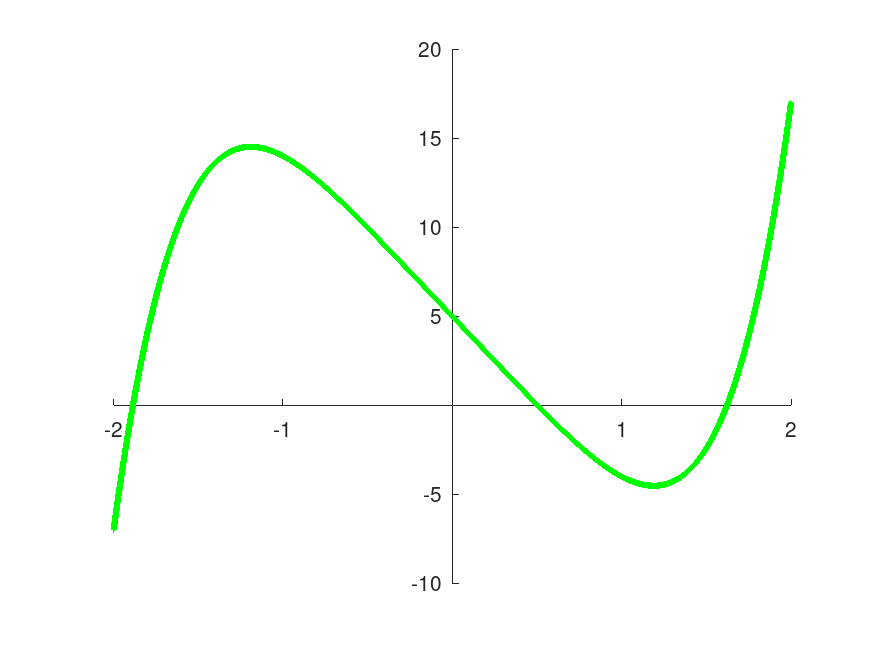
\includegraphics[width=8cm, height=3.5cm]{quantic2.png}
    \caption{\footnotesize Plotted by the ``GNU-Octave''}
  \end{figure}

 From its graph this polynomial has only three real roots. This polynomial is ``irreducible over \(\mathbb{Q}\) by the Eisenstein's criterion'' \cite{hunger} so by Theorem-12 its \textcolor{magenta}{Galois group is \(S_5\) which contains \(5!=120\) elements}.
\end{frame}

\begin{frame}{Galois Group of a seventh degree polynomial}
  The polynomial is \textcolor{green!50!black}{\(f(x)=x^7-2x^5-4x^3+2x^2+4x-2\)} which is ``irreducible over \(\mathbb{Q}\) by the Eisenstein's criterion'' \cite{hunger}. Its graph is shown below.

  \begin{figure}[h!]
    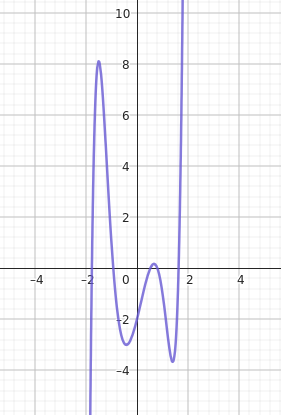
\includegraphics[width=8cm, height=3.5cm]{seventh2.png}
    \caption{\footnotesize Plotted by the ``Geogebra''}
  \end{figure}

  The Graph shows this polynomial has exactly five real roots. So exactly two of its roots are complex. Hence by the Theorem-12 its \textcolor{magenta}{Galois Group is \(S_7\) which contains \(7!=5040\) elements}.
\end{frame}

\subsection{Galois Groups of Multi-variable Poly.}
\begin{frame}{Galois Group of Multi-variable Polynomials}
  The Galois group of a polynomial in single variable can be generalized to the Galois group of a multi-variable polynomial.\\[3mm]
If the polynomial is \textcolor{green!50!black}{\(f(x,y)=x+y \in \mathbb{Q}[x,y]\)}. The roots of \(f\) span all over the complex numbers. Hence its \textcolor{magenta}{Galois group is \(\mathbb{C}\)}.


\vspace{2mm}
 \begin{tcolorbox}[colback=white, colframe=brown!80!black, boxsep=1mm, title={\bfseries \color{white} Example}]
  The polynomials in \(\mathbb{Q}[x,y]\) are: \begin{align}
                         y &= x^2+1 \\
                         y&=x
                       \end{align}
                       The roots of these simultaneous polynomials are \(\omega, {\omega}^2\). Then the splitting field of this system is \(\mathbb{Q}(\omega)\). Here the automorphisms of \(\mathbb{Q}(\omega)\) are: \\
       \(\omega \longmapsto \omega\) and \hspace{9mm} \(\omega \longmapsto {\omega}^2\).\\
                       \textcolor{magenta}{Hence the Galois group of this system is \(\{(1), (12)\} \cong {\mathbb{Z}}_2\)}.
\end{tcolorbox}
\end{frame}

\section{Application to the Classic Problem}
\subsection{Radical Extension}
\begin{frame}{Application to the Classic Problem}
  \begin{tcolorbox}[colback=white, colframe=red, boxsep=1mm, title={\bfseries \color{white} Question:}]

    \begin{enumerate}
    \item Is every polynomial equation solvable by the method of radicals?
    \item In other words; does there exist an explicit "formula" which gives all solutions of a polynomial equation?
    \end{enumerate}
  \end{tcolorbox}


\textcolor{violet}{If the degree of the polynomial is at most four then the answer is \textbf{yes} \cite{hunger}.}
\vspace{7mm}
\begin{definition}[Radical Extension]
  An extension field \(F\) of a field \(K\) is a radical extension of \(K\) if \(F=K(u_1,...,u_n)\), some power of \(u_1\) lies in \(K\) and for each \(i \geq 2\), some power of \(u_i\) lies in \(K(u_1,...,u_{i-1})\) \cite{hunger}.
\end{definition}
\vspace{4mm}
\textcolor{green!50!black}{The equation \(f(x)=0\) is \textit{solvable by radicals} if there exists a radical extension} \(F\) of \(K\) and splitting field \(E\) of \(f\) over \(K\) such that \(F \supset E \supset K\) \cite{hunger}.
\end{frame}

\subsection{Outcomes}
\begin{frame}{Some Results}

  \begin{theorem}[Theorem]
If \(F\) is a radical extension of \(K\) then \(Aut_K^F\) is a solvable group \cite{hunger}.
\end{theorem}

\begin{corollary}[Corollary]
If the equation \(f(x)=0\) is solvable by radicals, then the Galois group of \(f\) is a solvable group \cite{hunger}.
\end{corollary}

\begin{theorem}[Theorem]
The symmetric group \(S_n\) is not solvable for \(n \geq 5\) \cite{hunger}.
\end{theorem}

  \begin{tcolorbox}[colback=white, colframe=red, boxsep=1mm, title={\bfseries \color{white} Outcomes}]
  The polynomial \(f(x)=x^5-10x+5 \in \mathbb{Q}[x]\) has Galois group ``\(S_5\), which is not a solvable group'' \cite{hunger}. \\
The quantic polynomials over \(\mathbb{Q}\) are not solvable by radicals. That is there does not exist an explicit formula for solving the quantics. \\
Moreover, \textcolor{green!50!black}{polynomials of degree \(n \geq 5\) are not solvable by radicals} \cite{hunger}.
\end{tcolorbox}

\end{frame}

\subsection{Illustrations}
\begin{frame}[allowframebreaks]{Illustrations}
  Galois theory gives the precise condition under which a polynomial of degree \(n \geq 5\) is solvable by radicals or not.

  \vspace{7mm}
   \begin{tcolorbox}[colback=white, colframe=brown!80!black, boxsep=3mm, title={\bfseries \color{white} Example}]
  The polynomial is \(x^5-1 \in \mathbb{Q}[x]\).\\
  The set of  roots of this polynomial are the fifth roots of unity which forms a group under addition modulo \(5\). Hence the \textcolor{violet}{Galois group is isomorphic to \(\mathbb{Z}_5\)} \cite{hunger}. The group \(\mathbb{Z}_5\) is cyclic and ``every cyclic group is solvable'' \cite{galois}. Hence this polynomial is solvable by radicals.
\end{tcolorbox}

\framebreak
\begin{definition}[Cyclotomic Polynomial]
 The \(nth\)-cyclotomic polynomial is the polynomial \({\Phi}_n\) defined as \({\Phi}_n= \prod {(x-\zeta)}\), where \(\zeta\) is a primitive-\(nth\) of unity \cite{galois}.
\end{definition}

\begin{theorem}[Theorem]
  The Galois group of a \(nth\)-cyclotomic polynomial \({\Phi}_n\) of is \(\mathbb{Z}_n\) \cite{galois}.
\end{theorem}

\vspace{5mm}
 \begin{tcolorbox}[colback=white, colframe=brown!80!black, boxsep=1mm, title={\bfseries \color{white} Example}]
The polynomial is \(f(x)=x^{12}-x^{10}+x^8-x^6-x^2+1 \in \mathbb{Q}[x]\) \cite{galois}\\
which is a 58th-cyclotomic polynomial i.e this polynomial \(f(x)={\Phi}_{58}\).\\
So its \textcolor{violet}{Galois group is \(\mathbb{Z}_{58}\)}, which is abelian and hence is solvable. Therefore this polynomial \(f(x)\) is solvable by radicals.
\end{tcolorbox}
\end{frame}

\section{Galois Field}
\subsection{Representation of Galois Fields}
\begin{frame}{Galois Fields}
  Galois fields are the finite fields. We denote Galois field with \(q\) elements by \(GF(q)\).\\[4mm]

\textcolor{red}{\textbf{Integer representation}}\\[2mm]
\(GF(p^n)=\{0,1,...,p-1\} \cup \{p,p+1,...,p+p-1\} \cup ... \cup \{p^{n-1},p^{n-1}+1,...,p^{n-1}+p^{n-2}+...+p-1\}\) \cite{galois}.
\vspace{5mm}

\begin{example}[Example]
    \(GF(2)=\{0,1\}\)\\
    \(GF(2^3)=\{0,1\} \cup \{2,2+1\} \cup \{2^2,2^2+1,2^2+2,2^2+2+1\}=\{0,1,2,3,4,5,6,7\}\)
\end{example}
\end{frame}

\begin{frame}{Operations in Galois Field}
\textcolor{red}{\textbf{Polynomial representation}}\\[2mm]
If \(F\) is a finite field and \(f(x) \in F[x]\) is irreducible then \textcolor{green!50!black}{\(F[x]/(f(x))\) is finite field \cite{galois}.} This field consists of all polynomials modulo \(f(x)\). \\
If \(F=GF(2^3)\) then \textcolor{green!50!black}{\(f(x)=x^8+x^7+...+x+1 \in F[x]\)} is irreducible in \(F[x]\). Since \(F\) has \(8\) elements which are modulo \(8\), elements of \(F\) is represented by the elements of the factor ring \(F[x]/(f(x))\) \cite{aes}. \\[5mm]


In the Example-19, the number \(5\) has the representation \(2^2+1\). This gives the polynomial representation \(x^2+1=(101)\)(coefficient of \(x^2\) is \(1\) of \(x\) is \(0\) and of constant is \(1\) ) Now the binary equivalent of \(5\) is \(101\).\\[5mm]

\textcolor{red}{\textbf{Operations in Galois Field}}\\[2mm]
Let the Galois field be \(GF(p^n)\). Since the elements of a Galois field can be represented as polynomials the operations are similar to polynomial operations.
\end{frame}

\section{Application to Coding Theory}
\subsection{Error Correcting Codes}
\begin{frame}{Coding Theory}
  Any information gets deteriorated or lost over time.

\begin{enumerate}
\item Paintings gets deteriorated over time and has to be renovated.
\item Some of the words spoken by teacher in the class is missed due to noise \cite{coding}.
\end{enumerate}
\vspace{3mm}
\textcolor{violet}{The loss of information is inevitable.}
\begin{itemize}
\item To be able to over come this issue , i.e \textcolor{green!50!black}{to be able to detect and correct errors during transmission} of information in digital system "coding theory" is developed. In digital system, information are transmitted as strings of \(0\) and \(1\).

\item So \textcolor{green!50!black}{the fundamental of the coding theory in digital system is the manipulation of strings of binary digits}. The proper and complete manipulation of these strings is possibly only if the space of the strings is a field. This field is finite so this field is a \textbf{Galois field}. This is where the application of Galois theory comes.
  \end{itemize}
\end{frame}

\begin{frame}{Error Correcting Codes}
  The idea of coding theory is to append some extra digits to the information and use this to detect and possibly correct the errors during transmission.  These codes \textcolor{green!50!black}{that can correct themselves are called} \textcolor{magenta}{Error correcting codes} \cite{coding}.
  \vspace{3mm}


\begin{definition}[Linear Code]
Let \(K=GF(q)\) be a Galois field. Then a finite extension of \(K\) of dimension \(n\) is \(V=GF(q)^n=GF(q^n)\).\\
  \textcolor{violet}{A linear code \(C\) is a subspace of \(V\).} The code \(C\) has dimension \(k \leq n\) and the length \(n\). It is called a \((n,k)\) code \cite{error_correct}.
\end{definition}

  \begin{tcolorbox}[colback=white, colframe=blue!40, boxsep=1mm]
\textcolor{violet}{The usefulness of linear code is that they are vector spaces over the base field} so they have a basis. All the code words can be generated with this basis. Instead of storing all \(2^k\) number of code words (for \(k\)-dimensional binary codes), storing only \(k\) basis elements is sufficient which saves massive storage.
\end{tcolorbox}
\end{frame}

\begin{frame}{Illustration}
  To apply \((n,k)\) coding first we need to group our information into blocks of length \(k\).
\(u_1,...,u_k\),  \(u_k,...,u_{2k}\),... . This space has dimension \(k\). Now these block of codes are encoded separately each to a code of length \(n\) as shown \cite{coding}.

\vspace{5mm}
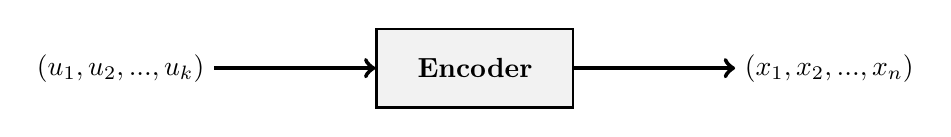
\begin{tikzpicture}
  \node [] (u) {\((u_1,u_2,...,u_k\))};
  \node[
  right of=u,
  rectangle,
  draw,
  thick,
  fill=gray!10,
  minimum width=25mm,
  minimum height=10mm,
  xshift=35mm] (e) {\bfseries Encoder};

  \node[right of=e, xshift=35mm] (x) {\((x_1,x_2,...,x_n)\)};

  \draw[->,ultra thick] (u)--(e);
  \draw[->,ultra thick] (e)--(x);
\end{tikzpicture}

\vspace{4mm}
\noindent
Mathematically, \textcolor{violet}{the encoded vector \(x\) is obtained form the original vector \(u\) using the generator matrix \(G\)} \textcolor{green!50!black}{by the relation \(x=uG\)} \cite{coding}.\\ To continue and complete the diagram.\\

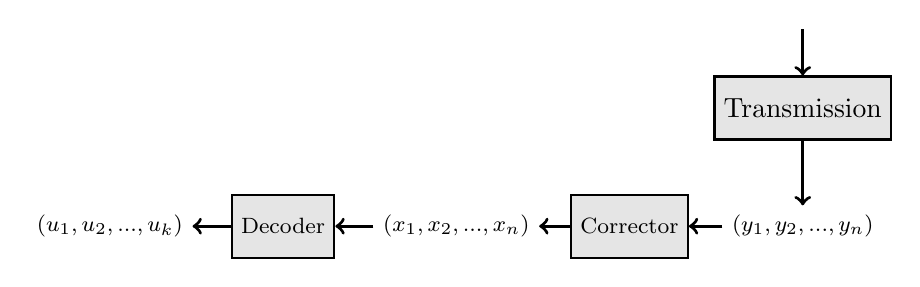
\begin{tikzpicture}
  \node[
  rectangle,
  draw,
  thick,
  fill=gray!20,
  minimum width=13mm,
  minimum height=8mm,
  ] (t) {Transmission};

  \node[below of=t, yshift=-5mm] (y) {\footnotesize \((y_1,y_2,...,y_n\))};

  \node[
  left of=y,
  rectangle,
  draw,
  thick,
  fill=gray!20,
  minimum width=13mm,
  minimum height=8mm,
  xshift=-12mm] (c) {\footnotesize Corrector};

  \node[left of=c, xshift=-12mm] (x) {\footnotesize \((x_1,x_2,...,x_n)\)};

  \node[
  left of=x,
  rectangle,
  draw,
  thick,
  fill=gray!20,
  minimum width=13mm,
  minimum height=8mm,
  xshift=-12mm] (d) {\footnotesize Decoder};

  \node[left of=d, xshift=-12mm] (u) {\footnotesize \((u_1,u_2,...,u_k\))};


  \draw[->,very thick] (0,1)--(t);
  \draw[->,very thick] (t)--(y);
  \draw[->,very thick] (y)--(c);
  \draw[->,very thick] (c)--(x);
  \draw[->,very thick] (x)--(d);
  \draw[->,very thick] (d)--(u);
\end{tikzpicture}
\end{frame}

\subsection{Decoding Process}
\begin{frame}{Syndrome Decoding}
  \begin{definition}[Syndrome of a code]
  The syndrome of a vector \(y \in V\) is defined as \\ \(syn(y)=\begin{pmatrix}
    y.h_1\\
    y.h_2\\
    ...\\
    y.h_{n-k}
  \end{pmatrix}\), \hspace{12mm} where \(\begin{pmatrix}
    h_1 \\ h_2\\ ...\\ h_{n-k}
  \end{pmatrix}\) is the \textcolor{violet}{parity check matrix} of \(C\). {\footnotesize A generator matrix \(H\) of the dual code \(C^{\perp}\) of the code \(C\) called a parity check matrix \cite{error_correct}}.
 \end{definition}
 \begin{tcolorbox}[colback=white, colframe=brown!80!black, boxsep=0mm, title={Decoding Process}]
 Suppose the signal received is the vector \(y\).
\begin{enumerate}
\item First we determine its syndrome, \(syn(y)\).
\item Determine the co-set of \(C\) containing \(syn(y)\), say \(e + C\).
\item Then \(y=e+x\) for some \(x \in C\). This implies \(x=y-e\). Since \(x \in C\), this \(x\) is the required decoding of \(y\) \cite{error_correct}.
\end{enumerate}
\end{tcolorbox}
\textcolor{violet}{This \(e\) is also called "error vector" \cite{error_correct}.}

\end{frame}

\begin{frame}{An example}
Suppose we have the parity check matrix is \(H=\begin{pmatrix}
    1 & 1 & 1 & 0\\
    0 & 1 & 0 & 1
  \end{pmatrix}\) and the code is   \(C=\{(0,0,0,0),(1,0,1,0),(0,1,1,1),(1,0,1,1)\} \;\; \subset GF(2^{4})\).\\[5mm]

  \textcolor{violet}{Suppose the received vector is \(y=(1,1,1,0)\)}. Then \(y \not \in C\) so the information is distorted from the original information. To get the original information:\\
  \(syn(y)= \begin{pmatrix}
    y.h_1 \\ y.h_2
  \end{pmatrix} = \begin{pmatrix}
    1 \\ 1
  \end{pmatrix}\) \\
  where \(h_1\) is the first row and \(h_2\) is the second row of \(H\).\\[5mm]
  Now \textcolor{violet}{if \(e=(0,1,0,0)\)} then \(e+C=\begin{pmatrix}
    1 \\ 1
  \end{pmatrix}\) so \(y-e=(1,1,1,0)-(0,1,0,0)=(1,0,1,0) \in C\) is the original information \cite{error_correct}.
\end{frame}
\subsection{Usages}
\begin{frame}{Some Usages}
  \begin{enumerate}
  \item The \((3,1)\) binary code is used in the short-range wireless communication system like \textcolor{blue}{\(Bluetooth^{TM}\)} \cite{wireless}.

    \vspace{3mm}
  \item The Hamming Code \((7,4)\) is used in \textcolor{violet}{memory devices like RAM} \cite{coding}.

\vspace{3mm}
  \item The Cyclic codes are used in storing data in \textcolor{green!50!black}{CDs and DVDs} \cite{coding}.
  \end{enumerate}
\end{frame}

\section{Application to Cryptography}
\subsection{Advance Encryption Standard}
\begin{frame}{Application to Cryptography}
  Cryptography is the science of \textcolor{violet}{safe-guarding information} by converting the original information into something unreadable. Galois Fields are the life of modern cryptography used in digital communication.
  \vspace{3mm}

  \begin{tcolorbox}[colback=white, colframe=brown!80!black, boxsep=1mm, title={Advance Encryption Standard(AES)}]
    The Advance Encryption Standard is a Computer Security Standard for cryptography which is approved by the ``Federal Information Processing Standards Publications'' of USA which became effective on May 26, 2002.
  \end{tcolorbox}

\vspace{3mm}
In 2000, NIST announced the selection of the ``Rijndael'' block cipher family which was developed by \textcolor{violet}{two Belgian cryptographers, \textit{(Vincent Rijmen and Joan Daemen)}} as the winner of the AES competition and since then AES has been the standard for digital cryptography.
\end{frame}

\begin{frame}[allowframebreaks]{Algorithm}
  The generic algorithm of AES consists of smaller sub-algorithms namely \textcolor{green!50!black}{Sub-Bytes, Shift-Rows, Mix-Columns and Add-Round-Key} \cite{aes}.
\vspace{2mm}
  \begin{enumerate}
  \item \textbf{\textcolor{blue}{The State}}\\
    First the data is broken into blocks, each of size 16 byte. \textcolor{violet}{Each block is then represented in a \(4 \times 4\) matrix, whose each entry is a byte of the block}. This matrix is called the State.\\
    Suppose the block is \(b_1, b_2,...,b_{16}\). Then the state is
    \(\left[\begin{smallmatrix}
  b_1 & b_5 &... & ...\\
  b_2 & b_6 &... & ...\\
  b_3 & b_7 &... & ...\\
  b_4 & b_8 &... & b_{16}
\end{smallmatrix}\right]\)
\vspace{2mm}

    Mathematical operations are not applicable to the data directly so the significance of this step is to make the data applicable for mathematical operations.
  \item \textbf{\textcolor{blue}{Sub-Bytes}}\\
    In this step, first each byte of the matrix is replaced with its \textcolor{violet}{multiplicative inverse} if it has one. Then it transforms each bytes using an invertible \textcolor{violet}{affine transformation, \(x \mapsto Ax+b\)} \cite{aes}.\\
    \framebreak
    \textcolor{magenta}{Mathematical Preliminaries}\\
    Each byte in the state i.e each entry in the matrix, is interpreted as one of the 256 elements of a finite field \(GF(2^8)\). Then the addition, multiplication operations are performed according to the respective field operations of the field \(GF(2^8)\).
\vspace{2mm}
    \item \textbf{\textcolor{blue}{Shift-Rows}}\\
In this step entries of a row is shifted to scramble data. \textcolor{violet}{Row-n shifted to the left by \(n-1\) unit}. Here,\\
\(1-1=0\), so row-1 is left unchanged. \(2-1=1\), so row-2 is shifted to the left by 1 unit and row-3 by 2 unit and so on as shown below \cite{aes}.\\
\vspace{3mm}
If \(A=\begin{bmatrix}
    a_{11}&a_{12}&a_{13}&a_{14}\\
    a_{21}&a_{22}&a_{23}&a_{24}\\
    a_{31}&a_{32}&a_{33}&a_{34}\\
    a_{41}&a_{42}&a_{43}&a_{44}
    \end{bmatrix}\) \hspace{3mm} then \(A'=\begin{bmatrix}
    a_{11}&a_{12}&a_{13}&a_{14}\\
    a_{22}&a_{23}&a_{24}&a_{21}\\
    a_{33}&a_{34}&a_{31}&a_{32}\\
    a_{44}&a_{41}&a_{42}&a_{43}
  \end{bmatrix}\) \vspace{2mm} \\[3mm] is the matrix after Shit-Row

    \framebreak

  \item \textbf{\textcolor{blue}{Mix-Columns}}\\
    In this step \textcolor{violet}{each column is transformed using a linear transformation, \(c \mapsto Bc\)} where \(c\) is a column of the matrix obtained above. Since linear transformation is invertible this step is invertible. Note every step of this algorithm must be invertible to be able to decrypt the data \cite{aes}.

    \vspace{5mm}

  \item \textbf{\textcolor{blue}{Add-Round-Key}}\\
This is the step where the encrypted data gets uniqueness. \textcolor{violet}{Each user is assigned an "unique key"} and this key is added to the matrix obtained from the last step \cite{aes}.
  \end{enumerate}
\end{frame}

\begin{frame}[allowframebreaks]{Illustration}
  Let us encrypt the sentence \textcolor{violet}{Fun Cryptography}. This consists of exactly 16 characters.\vspace{2mm}

\begin{enumerate}
\item First we write the ASCII representation of each character of the sentence as shown below. We do so because the ASCII representation gives the binary representation of each character which has a size of a byte. \textcolor{violet}{The ASCII representation of "F" is \(70\) which is \(01000110\) in binary}.\vspace{2mm}

  \[\hspace{-3mm} \begin{bmatrix}
      70 & 117 & 110 & 32 \\
      67 & 114 & 121 & 112\\
      116 & 111 & 103 & 114 \\
      97 & 112 & 104 & 121
    \end{bmatrix}=
    \begin{bmatrix}
      01000110 & 01110110 & 01101110 & 00010000 \\
      01000011 & 01110010 & 01111001 & 01110000\\
      01110100 & 01101111 & 01100111 & 01110010 \\
      01100001 & 01110000 & 01101000 & 01111001
    \end{bmatrix}
  \]
\item After performing Sub-Bytes, Shift-Rows, Mix-Columns, we get the following matrix.

  \framebreak
  \[\hspace{-5mm}\begin{bmatrix}
      11100111 & 00011000 & 00100100 & 01110000\\
      00101010 & 10101011 & 00111001 & 01100011\\
      00010101 & 01100101 & 11110111 & 10100111\\
      10101011 & 11110110 & 00000011 & 10100100
    \end{bmatrix}=
    \begin{bmatrix}
      231 & 24 & 36 & 112\\
      42 & 171 & 57 & 99\\
      21 & 101 & 247 & 167\\
      171 & 246 & 3 & 164
    \end{bmatrix}
  \]
  \vspace{5mm}

\item We have omitted the Add-Round-Key step just for the sake of simplicity. The matrix obtained at last in step-2 translates to something different from our original sentence.

  \vspace{5mm}

\item The decryption process is applying the inverse of the encryption process \cite{aes}.
\end{enumerate}
\end{frame}
% ------------------------------------------------------------------------------------------------------------------

\section{References}
\subsection{References}
\begin{frame}{References}
  \footnotesize

  \begin{thebibliography}{9}

  \bibitem{galois}
    J. P. Escofier. \emph{Galois Theory}. Springer, New York:219-225,2000.

  \bibitem{error_correct}
    G. R. Holdman. \emph{Error Correcting Codes  Over Galois Rings}. Graduate Dissertation, Department of Mathematics, Whitman college, 345 Boyer Ave.
    Walla Walla, Washington, U.S.A, 2019.

  \bibitem{hunger}
    T. W. Hungerford. \emph{Algebra}. Springer (India), New Dheli, 2012.

  \bibitem{algorithm}
    A. Lenstra, H. Lenstra, and L. Lovasz. Factoring polynomials with rational coefficients. \emph{Mathematische Annalen},261,12,1982.

  \bibitem{coding}
    A. Neubaer and J. Freudenberger and V. Kuhn. \emph{Coding Theory, Algorithms, Architectures, and Applications}. John Wiley and Sons Ltd, Chichester, West Sussex, England:1-93,2007.

  \bibitem{wireless}
    D. Sarma. Implementation of Galois Field for Application in Wireless Communication Channels. \emph{MATEC Web of Conferences},2010:03012,2018.

  \bibitem{aes}
    National Institute of Standards and Technology. Advanced Encryption
    Standard (AES). \emph{(Department of Commerce, Washington, D.C.), Federal Information Processing Standards Publication (FIPS) NIST FIPS}. 197-upd1, 2001. updated May 9, 2023. doi:10.6028/NIST.FIPS.197-upd1.
  \end{thebibliography}
\end{frame}

\subsection{Acknowledgments}
\begin{frame}{Acknowledgments}

  First of all I would like to thank my \textbf{supervisor} Assoc. Prof. \textcolor{blue}{Tulasi Prasad Nepal}. Then I am thankful to former HOD of the department Prof. Dr.\\
  \textcolor{violet}{Tanka Nath Dhamala} for his support and time.\\[4mm]

I am grateful to Kathmandu Center for Research and Education Chinese Academy of Sciences-TU for awarding me with \\
\textcolor{violet}{KCRE Excellent Student Thesis Grant 2023(Grant number: 08092023).}\\[4mm]

I would like thank  Mr. \textcolor{green!50!black}{Santosh Gnawali} for providing me the necessary articles and to Mr. \textcolor{green!50!black}{Dipak Babu Amgain} for assisting me with the bibliography and to Dr. \textcolor{green!50!black}{Bishnu Hari Subedi} for helping me to write an article. Finally I am thankful to the HoD of the CDM  Prof. Dr. \textcolor{green!50!black}{Chet Raj Bhatta} for organizing this defence in time.
\\[4mm]
\begin{center}
  \large \bfseries \color{magenta}
  Thank You
  \end{center}
\begin{minipage}{1\textwidth}
	\begin{flushright}
		%
		{\color {blue} Sandesh Thakuri}\\
		%
	\end{flushright}
      \end{minipage}
\end{frame}
\end{document}




%%% Local Variables:
%%% mode: latex
%%% TeX-master: t
%%% End:
